\begin{Example}[berkeley9]{Berkeley admissions}
These diagnostic plots may also be illustrated
with the Berkeley admissions
data using the \loglin\ model $[AD] [GD]$,
or the equivalent logit model, $\logit(\mbox{Admit}) = \alpha + \beta_i^{D}$.
Recall that we found this model fit well, except in department A.
To give useful labels for influential cells, we first combine the
factor variables into a character identifier, \pname{cell}.
\begin{listing}
data berkeley;
   set berkeley;
   cell = trim(put(dept,dept.)) ||
          gender ||
          trim(put(admit,yn.));
\end{listing}
We ask for an influence plot of adjusted Pearson residuals against hat values
(showing Cook's D by bubble size, by default):
\begin{listing}
%inflglim(data=berkeley, class=dept gender admit,
        resp=freq, model=admit|dept gender|dept, dist=poisson, id=cell,
        gx=hat, gy=streschi);
\end{listing}
The plot (\figref{fig:genberk11}) clearly indicates that the only cells
which do not fit ($|r_i| > 2$) are for department A.
Notice also, that the cells for males applying to this department
(with high expected frequencies)
have large leverage, and therefore large influence (Cook's D)
on this model.
%% one figure
\begin{figure}[htb]
  \centering
  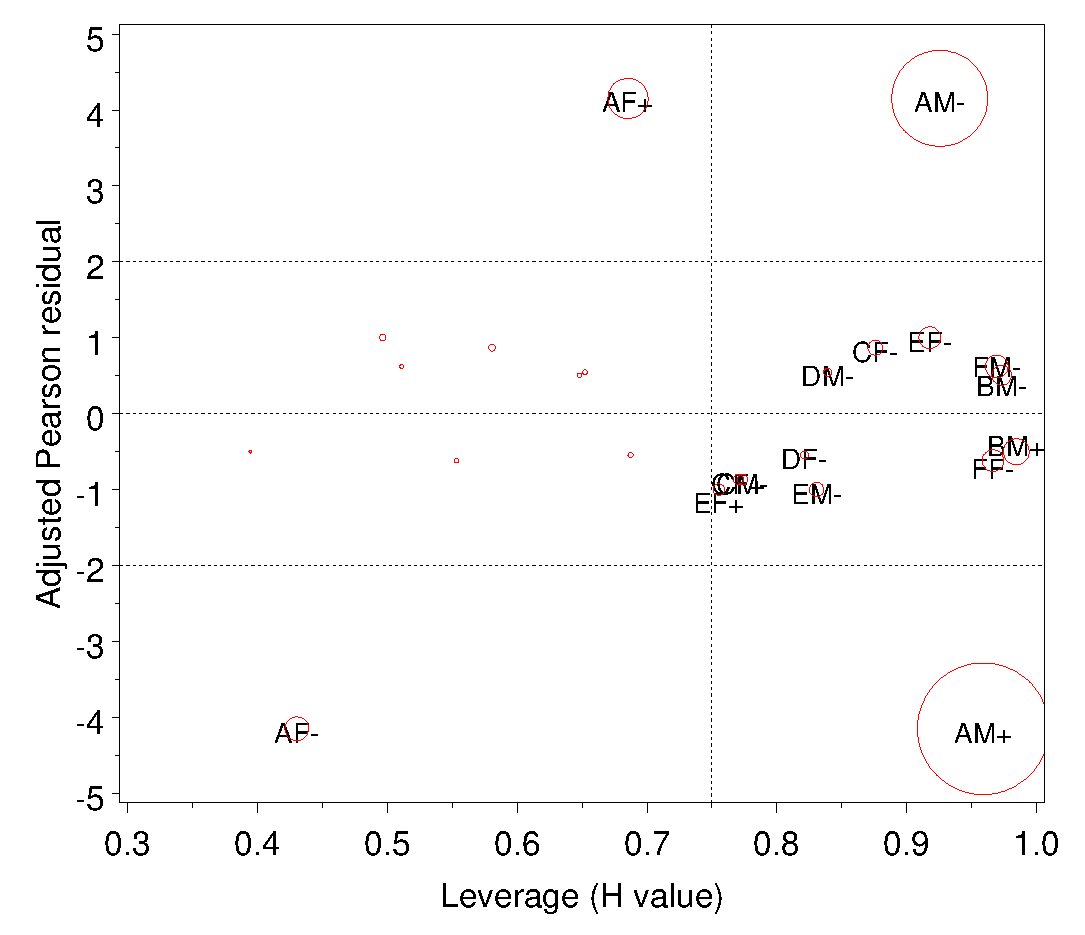
\includegraphics[scale=.6]{genberk11}
  \caption[Influence plot for Berkeley admissions data, Model AD GD]{Influence plot for Berkeley admissions data, Model $[AD] [GD]$.
  Bubble areas are proportional to Cook's D.}%
  \label{fig:genberk11}
\end{figure}

We can also illustrate why adjusted residuals are preferable to
the (crudely standardized) residuals by plotting the estimated
residual standard error, $\sqrt{1-h_{ii}}$ against fitted cell
frequency for this model.
This plot (\figref{fig:genberk12}) is produced as follows:
\begin{listing}
%inflglim(data=berkeley, class=dept gender admit,
        resp=freq, model=dept|gender dept|admit, dist=poisson, id=cell,
        gx=pred, gy=seres);
\end{listing}

%% one figure
\begin{figure}[htb]
  \centering
  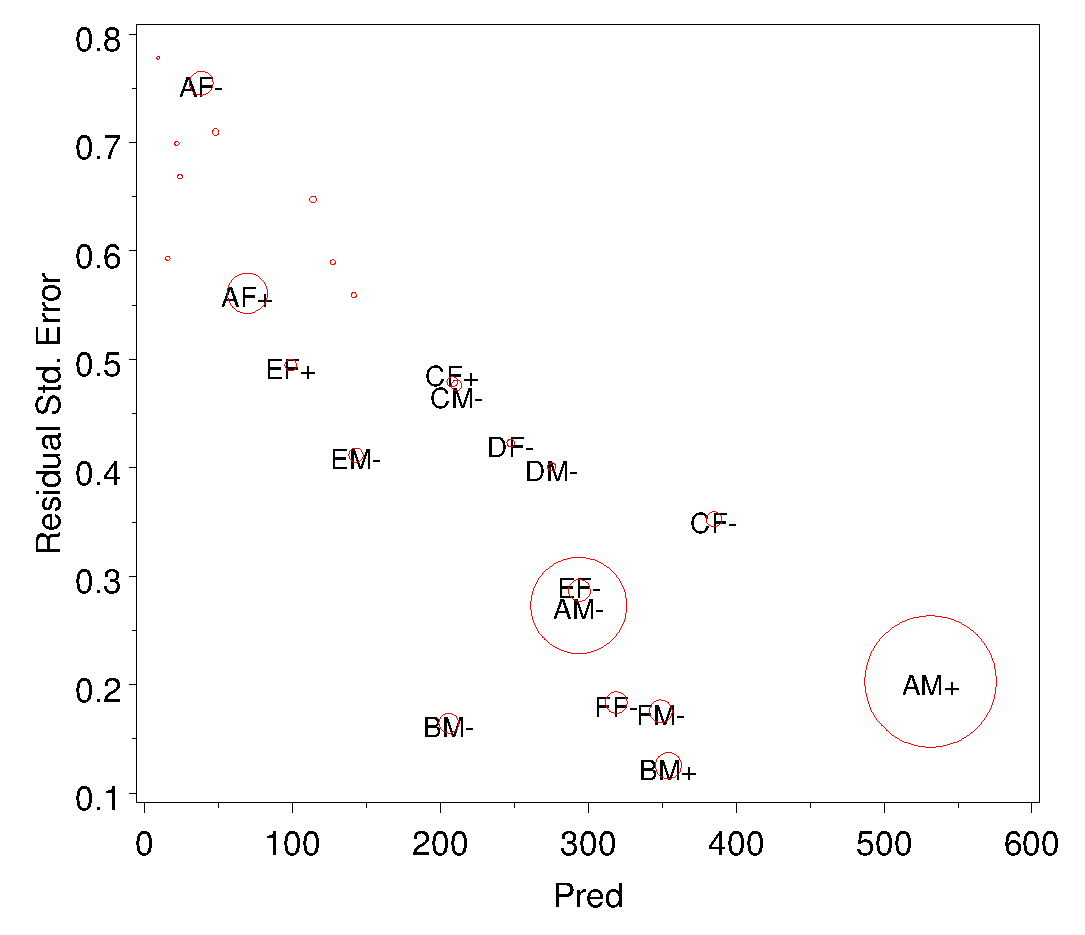
\includegraphics[scale=.6]{genberk12}
  \caption[Residual standard errors vs.\ fitted frequencies]{Residual standard errors vs.\ fitted frequencies for Berkeley admissions data, Model $[AD] [GD]$}%
  \label{fig:genberk12}
\end{figure}
We see that the standard errors decrease nearly linearly
with estimated expected frequency,
and the most influential cells (\pname{AM+} and \pname{AM-} for
males in Dept A)  have small standard errors,
and so their unadjusted residuals are most severely underestimated.
That is, cells with large expected frequency are
often highly influential, but their (unadjusted) residuals are
underestimated. 

Finally, we show a half-normal plot for this model in \figref{fig:genberk13},
produced with the \macro{HALFNORM},
\begin{listing}
%halfnorm(data=berkeley, class=dept gender admit,
   resp=freq, model=dept|gender dept|admit, dist=poisson, id=cell);
\end{listing}
By default, the cells with the largest 5 absolute residuals are labeled.
This plot clearly shows that the model fits well, except in department A.
%% one figure
\begin{figure}[htb]
  \centering
  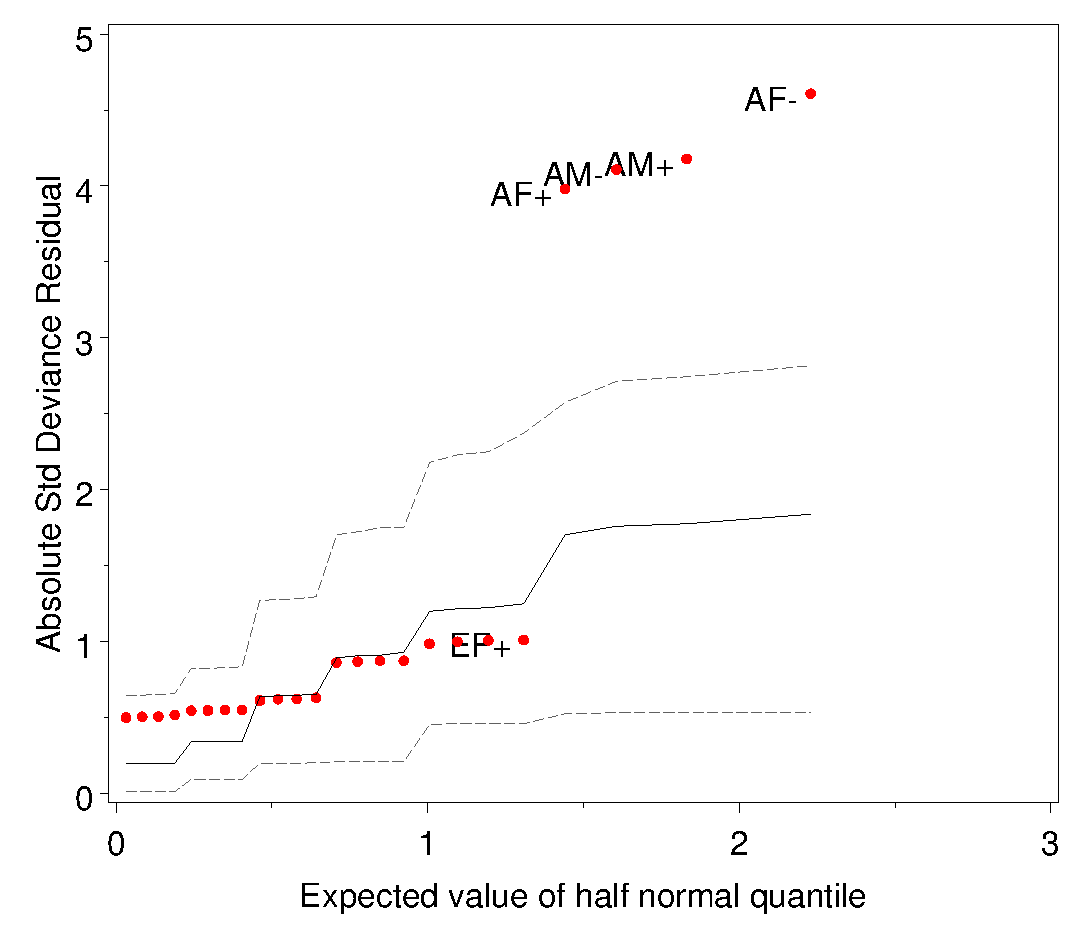
\includegraphics[scale=.6]{genberk13}
  \caption{Half-normal residual plot for Berkeley admissions data, Model $[AD] [GD]$}%
  \label{fig:genberk13}
\end{figure}
\end{Example}
